\documentclass[UTF8,a4paper,11pt,fontset=none]{ctexart}
\IfFileExists{C:/Windows/Fonts/simsun.ttc}{%
  \setCJKmainfont[Path=C:/Windows/Fonts/,FontIndex=0,AutoFakeBold=2]{simsun.ttc}
  \setCJKsansfont[Path=C:/Windows/Fonts/,AutoFakeBold=2]{simhei.ttf}
}{%
  \setCJKmainfont[BoldFont=FandolSong-Bold.otf]{FandolSong-Regular.otf}
  \setCJKsansfont[BoldFont=FandolHei-Bold.otf]{FandolHei-Regular.otf}
}
\usepackage[margin=24mm,top=20mm,bottom=20mm]{geometry}
\usepackage{amsmath,graphicx,booktabs,url}
\setlength{\parindent}{2em}
\setlength{\parskip}{3pt}
\linespread{1.12}
\pagestyle{plain}
\ctexset{paragraph={runin=false,beforeskip=0.55ex,afterskip=0.22ex}}
\newcommand{\FourRows}{
CNN A & 89.7523 & 89.8202 & 0.290570 & 27,270 & 7/15 & CPU \\
GRU B & 91.8222 & 91.9444 & 0.255319 & 14,790 & 23/30 & CPU \\
Transformer C & 88.0896 & 88.0326 & 0.425905 & 34,502 & 7/15 & CPU \\
Mamba D & 88.7004 & 88.8610 & 0.379041 & 33,670 & 3/11 & RTX 3090 \\
}
\newcommand{\AblationRows}{
42 & 89.8202 & 89.7161 & 89.6185 & -0.1041 & +0.0976 \\
43 & 88.5241 & 91.1212 & 92.1449 & +2.5970 & -1.0238 \\
44 & 90.0424 & 89.5221 & 88.6817 & -0.5204 & +0.8404 \\
}
\newcommand{\AblationStats}{
A & 89.4623 & 0.8200 \\
B & 90.1198 & 0.8726 \\
C & 90.1484 & 1.7914 \\
}
\newcommand{\GruRows}{
42 & 91.2793 & 91.3919 & 0.362237 & 14 & 22 \\
43 & 89.7523 & 89.8447 & 0.313432 & 7 & 15 \\
44 & 90.7024 & 90.7504 & 0.352929 & 24 & 30 \\
均值 & 90.5780 & 90.6623 & 0.342866 & — & — \\
样本标准差 & 0.7711 & 0.7774 & 0.025912 & — & — \\
}

\title{\textbf{UCI HAR 时序活动识别}\\[4pt]\large 第四次学习规划最终归档}
\author{SequenceModel-HAR-Lab}
\date{2026 年 11 月 23 日}
\begin{document}
\maketitle

\begin{abstract}
本报告收录四模型 Seed42 基线、CNN 三种子配对消融、GRU Task03 GPU 三种子以及第四次学习规划第八部分的 48 道宏观理解题。GRU 在本次四模型基线中测试 Macro-F1 最高。SE 相对原 CNN 的均值提高主要由 Seed43 驱动。GRU Task03 的种子波动限于固定受试者划分。教师总体验收 48/48 依据任务提供的结论登记；逐字原答与逐题验收证据的可恢复范围另行注明。
\end{abstract}

\section{研究目标与任务}
以手机惯性信号为输入学习跨受试者活动分类，比较四个序列模型的具体实现、检验 CNN 通道重加权的收益，再用三次 GRU 运行观察随机初始化与采样顺序的联合变化。

\section{数据与预处理}
UCI HAR 使用 50 Hz 的九路惯性信号，每个窗口为 \(128\times9\)，覆盖 2.56 秒。标签为步行、上楼、下楼、坐、站和躺。使用官方时序窗口；561 维统计特征属于另一种表示。\cite{uci,protocol}

冻结集合为训练 6037 窗口／17 人、验证 1315／4、官方测试 2947／9，受试者互斥。只用训练集拟合逐通道参数，\(z=(x-\mu_{\rm train})/\sigma_{\rm train}\)。训练使用交叉熵并更新参数，验证以 Macro-F1 优先选模，同分比较 Loss。官方测试仅对选好的模型进行最终评价。

\section{序列模型与信息处理}
CNN 用一维卷积提取局部变化并经池化聚合。GRU 递归更新隐藏状态，由更新门和重置门调节信息传递，取末状态分类。Transformer 先投影并加位置编码，通过自注意力交换时间点信息，再平均聚合。官方 Mamba-1 用输入依赖的选择性状态空间更新，随后时间平均。四个模型均输出六类 logits。

\clearpage
\section{四模型 Seed42 基线}
表~\ref{tab:four} 取自各运行的指标、配置和训练归档。本次四个具体实现中 GRU 的 Accuracy 和 Macro-F1 最高，测试 Loss 最低。Mamba D 使用 Linux RTX 3090，另外三组为 CPU，耗时缺少共同硬件与计时口径。\cite{four}

\begin{table}[htbp]
\centering\small
\caption{四模型 Seed42 官方测试结果，轮数为最佳／实际。}\label{tab:four}
\begin{tabular}{lrrrrrl}
\toprule
模型 & Accuracy (\%) & Macro-F1 (\%) & Loss & 参数 & 轮数 & 设备 \\
\midrule
\FourRows
\bottomrule
\end{tabular}
\end{table}

\section{CNN 三种子消融}
A 使用 27,270 参数的原始 CNN。B 在时间平均前加入 SE，通过 \(128\to16\to128\) 的通道门控缩放特征；C 在池化后加入等参数残差 MLP。B 和 C 各增加 4,240 参数。B/C 新运行直接保存共享层初始化指纹与实际逐轮采样指纹。A42 使用历史指标，原训练没有这两类指纹。审计按原构造和确定性配置重建初始化并回放批次顺序，与 B42 的 15 轮和 C42 的 13 轮直接记录匹配。\cite{abl,trace}

\begin{table}[htbp]
\centering\small
\caption{CNN 三组测试 Macro-F1（\%）及同种子差值（百分点）。}\label{tab:ab}
\begin{tabular}{rrrrrr}
\toprule
Seed & A & B & C & B--A & B--C \\
\midrule
\AblationRows
\bottomrule
\end{tabular}
\quad
\begin{tabular}{lrr}
\toprule
组 & 均值（\%） & 样本 SD（百分点） \\
\midrule
\AblationStats
\bottomrule
\end{tabular}
\end{table}

表~\ref{tab:ab} 与图~\ref{fig:pair} 的三组配对中，B--A 仅 Seed43 为正，平均 +0.6575 个百分点。B--C 的平均为 \(-0.0286\) 个百分点。当前证据支持这三次运行的描述性比较，不能判定 SE 普遍有效或无效。B/C 同参数量，插入点和运算存在差异，因果解释仍需额外对照。

\begin{figure}[htbp]
\centering
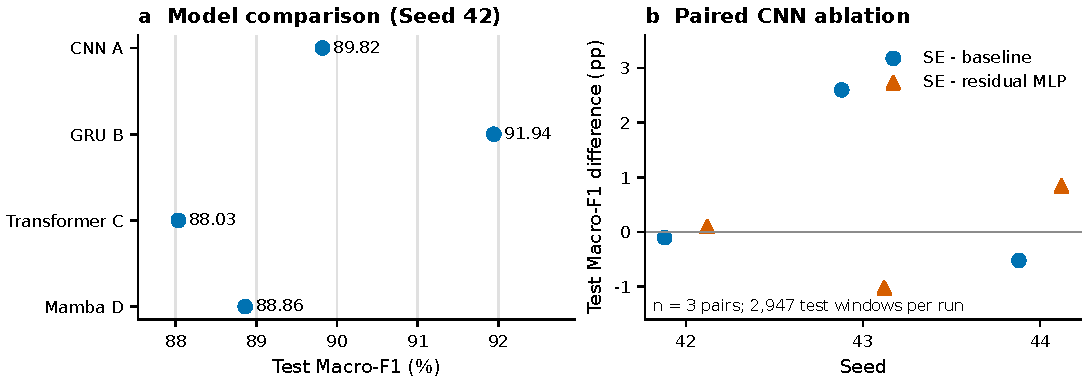
\includegraphics[width=0.96\linewidth]{../chapter06_lesson01_research_draft/results_figure.pdf}
\caption{归档的四模型 Macro-F1 与 CNN 配对差值。每个点来自实际历史运行；右图横线为零差值。}\label{fig:pair}
\end{figure}

\clearpage
\section{GRU Task03 三种子与错分}
Task03 三组采用 Ubuntu 24.04.3、RTX 3090、Python 3.9.23、PyTorch 2.5.1+cu121 与 NumPy 1.24.4。历史 CPU Seed42 采用 Windows 与 PyTorch 2.0.1，其 Macro-F1 为 91.9444\%，GPU Task03 Seed42 为 91.3919\%。操作系统、PyTorch 版本及后端共同变化，分数差异无法单独归因于设备。历史 CPU 指标和 Task03 GPU 指标分开保留。\cite{gru,task}

\begin{table}[htbp]
\centering\small
\caption{Task03 三次官方测试及样本标准差。Accuracy 与 Macro-F1 行单位为 \%，其标准差为百分点。}\label{tab:gru}
\begin{tabular}{lrrrrr}
\toprule
Seed & Accuracy & Macro-F1 & Loss & 最佳轮 & 实际轮 \\
\midrule
\GruRows
\bottomrule
\end{tabular}
\end{table}

表~\ref{tab:gru} 中 Seed43 的 Loss 最低，但 Accuracy 和 Macro-F1 也最低。交叉熵读真类概率，后两项使用硬预测。三个种子保持相同划分，Macro-F1 样本标准差为 0.7774 个百分点，只描述当前初始化与采样的联合波动。

\begin{figure}[htbp]
\centering
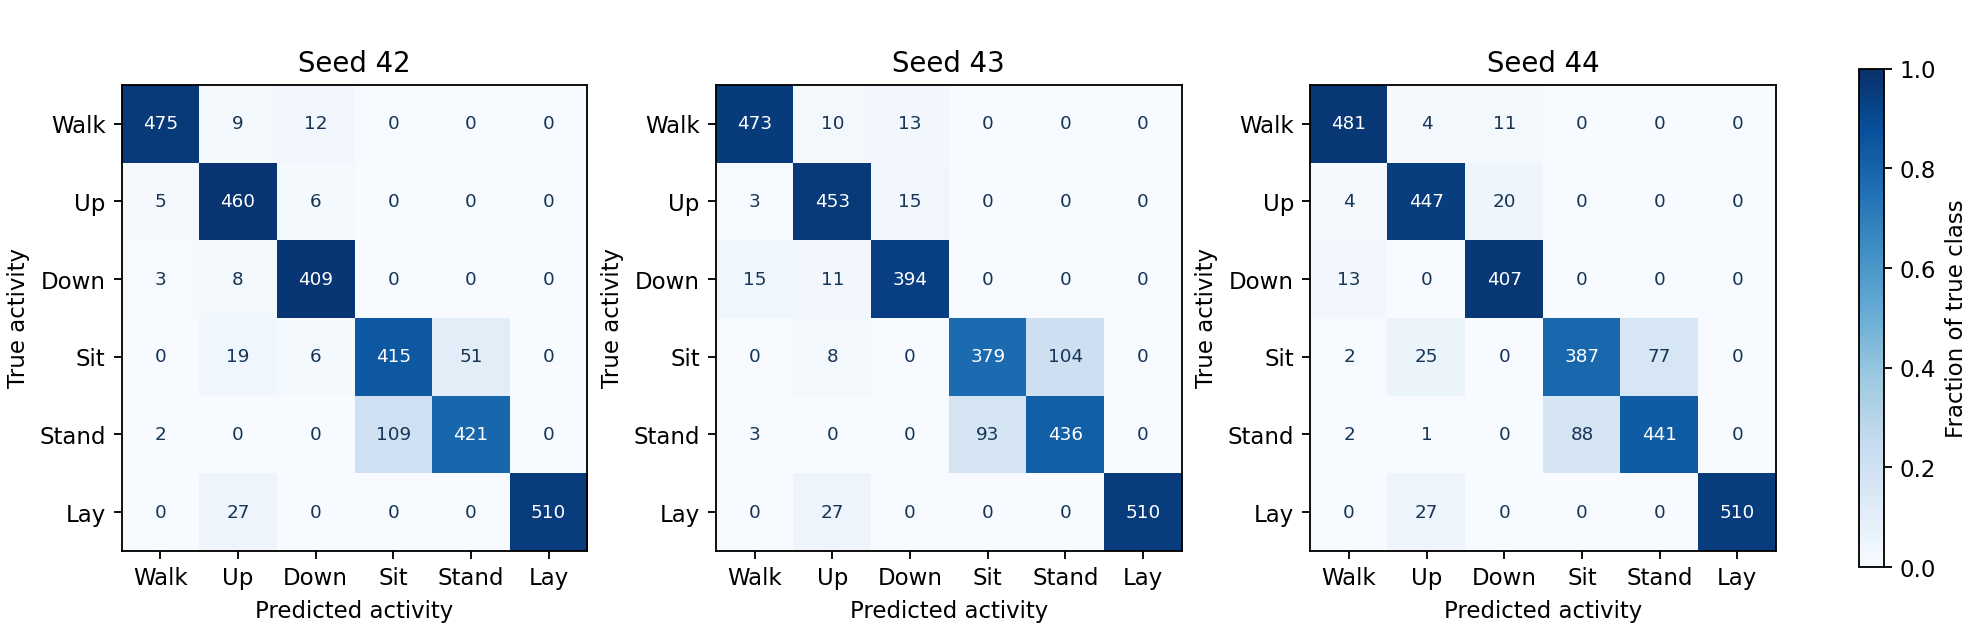
\includegraphics[width=\linewidth]{../gru_multiseed_task03_20261123/confusion_matrices.png}
\caption{Task03 原归档三种子混淆矩阵，行是真实类别，列是预测类别。}\label{fig:cm}
\end{figure}

图~\ref{fig:cm} 中，坐被预测为站的次数为 51、104、77，站被预测为坐为 109、93、88。SITTING 在三组均为最低 F1，跨种子跨度 3.06 个百分点；LAYING 每组均正确 510/537。这些计数和归档独立复算一致，逐样本预测留在服务器。坐站信号是否难以区分仍是待验证机制。

\clearpage
\section{Skill 工作流与科研证据}
Skill 定义任务流程，Script 执行具体操作，Experiment Record 保存实际运行证据。本次主动读取项目 Skill 完整指令后，按汇总路径交叉检查各基线原始记录、CNN 九组及 Task03 指标并编译报告。自动提供的 Skill 名称与路径只能证明元数据发现。复用档案中的训练指纹、检查点哈希和预测复算报告时，应分别标记同期记录、后续复核和当前可独立检查的范围。

Task03 三份 SHA256SUMS 共列出 60 个历史运行文件。此处可以复算公开副本的 18 项，Best/Last 的哈希与运行结果和清单交叉核对。其余 42 项包括实际权重、逐样本预测和原始日志，远程工作目录访问未成功，保留历史核验记录。数据、预测、权重均按项目约定留在各自环境。

\section{原规划 48 道宏观理解题}\label{sec:questions}
题目取自原规划 PDF 第 12--15 页。\cite{plan} 原版每组从 1 到 6 重新印刷编号，本文按各节定义的全局范围编号，CSV 同时保存两种编号。答案为依据学习或实验档案整理的最终理解。保存的 4 条学生原答来自 Day 01 同主题问答，引用处明确标识。教师 48/48 总评按任务提供的验收记录保留，个别原文缺口见逐题记录。下列简写可在证据索引中定位。

\begin{description}
\item[数据协议、Day 01 问答] 分割、训练集标准化、可取得的逐字学习记录。\cite{protocol,day}
\item[CNN 档案、历史 GRU 档案、Transformer 档案、四模型档案] 模型结构、配置、曲线及官方测试指标。\cite{cnn,gru,tr,four}
\item[CNN 消融、Seed42 复核、GRU Task03、Skill 调用] 配对、重建、三种子和执行记录。\cite{abl,trace,task,skill}
\end{description}
\clearpage\subsection{本轮训练任务与数据含义}
\paragraph{1. 本轮监督式活动分类想解决什么问题？请说明输入、标签和输出。}
输入是每个 128\(\times\)9 惯性信号窗口，监督标签是六类活动之一，输出是六个类别分数，经最大分数选出类别。\par
\textbf{历史证据}　未找到单题复测记录\par
\textbf{来源}　数据协议。原规划第 12 页。\par
\paragraph{2. 用一个UCI HAR窗口说明，128个时间点和9个通道分别表示什么。}
128 表示以 50 Hz 顺序采样的时间点，覆盖 2.56 秒；9 是总加速度、身体加速度和角速度的三轴信号，每一列对应一种轴向测量。\par
\textbf{历史证据}　未找到单题复测记录\par
\textbf{来源}　数据协议。原规划第 12 页。\par
\paragraph{3. 为什么一段信号的时间先后关系可能影响活动判断？}
相同的数值集合可以有不同的先后次序。步态的周期、转折及各轴之间的相位随顺序变化，打乱后会丢掉这类判别信息。\par
\textbf{历史证据}　未找到单题复测记录\par
\textbf{来源}　数据协议。原规划第 12 页。\par
\paragraph{4. 模型没有看到人的照片，为什么仍可能从传感器信号识别活动？}
走路时振荡、转身时的角速度和坐站时的姿态变化会在多通道中形成可学习的组合模式。无需假定每类存在独有特征。\par
\textbf{历史证据}　同主题学生原答：“因为从九路加速度和角速度信号中提取到独属于步行、坐下等活动的特征，分类出这些任务” 教师纠正：提醒“独属于”表述过强，应看多通道组合。 未找到单题复测记录\par
\textbf{来源}　Day 01 问答、数据协议。原规划第 12 页。\par
\paragraph{5. 判断六类活动与预测一个连续数值，在训练目标上有什么区别？}
六分类预测离散活动，通常用交叉熵；连续速度属于回归，可用均方误差等目标。分类与回归都属于预测。\par
\textbf{历史证据}　同主题学生原答：“任务A是分类任务，B是预测任务” 教师纠正：分类和回归都属于预测，后者预测连续数值。 任务提供的定向复测摘要为通过，逐字复答未提供。\par
\textbf{来源}　Day 01 问答、数据协议。原规划第 12 页。\par
\paragraph{6. 原始窗口信号与已经提取好的统计特征有什么区别，本轮使用哪一种？}
时序窗口保留逐时点的九路信号；561 维特征是事先计算的统计与频域摘要。本轮用官方已预处理的时序窗口。\par
\textbf{历史证据}　未找到单题复测记录\par
\textbf{来源}　数据协议。原规划第 12 页。\par
\clearpage\subsection{数据划分与预处理}
\paragraph{7. 训练集、验证集和测试集在本轮实验中分别承担什么职责？}
训练集更新参数，验证集用于选轮和早停，官方测试集仅用于最终评价。这里窗口数依次为 6037、1315、2947。\par
\textbf{历史证据}　未找到单题复测记录\par
\textbf{来源}　数据协议。原规划第 13 页。\par
\paragraph{8. 为什么按受试者划分，比把所有窗口随机打散更贴合本轮目标？}
目标是识别未见受试者的活动。按受试者隔离可以减少模型利用个人步态、手机位置等特征而高估跨人表现的机会。\par
\textbf{历史证据}　未找到单题复测记录\par
\textbf{来源}　数据协议。原规划第 13 页。\par
\paragraph{9. 同一人的相似或重叠窗口进入不同集合，会让评价产生什么问题？}
相邻窗口可能共用原始采样，随机跨集合会使验证或测试过于接近训练实例，产生乐观估计。官方相邻窗口有 50\% 重叠。\par
\textbf{历史证据}　未找到单题复测记录\par
\textbf{来源}　数据协议。原规划第 13 页。\par
\paragraph{10. 标准化怎样改变模型接收到的数据，为什么可能帮助训练？}
逐通道计算 z=(x\(\mathord{-}\)\(\mu\))/\(\sigma\)，使尺度更可比。例如 (14\(\mathord{-}\)10)/2=2。适当的缩放可能改善优化条件，训练误差或测试误差仍可能不降。\par
\textbf{历史证据}　同主题学生原答：“2，消除尺度太大导致的误差” 教师纠正：缩放可能减轻优化困难，不能保证误差下降。 Day 01 复测原答：防止尺度过大给优化带来困难。不是的。教师确认通过。\par
\textbf{来源}　Day 01 问答、数据协议。原规划第 13 页。\par
\paragraph{11. 为什么只用训练数据学习标准化参数，再应用于验证和测试数据？}
均值与标准差也是学习得到的参数。只从训练集估计可避免让评价数据影响预处理，同时保证三集合按同一尺度转换。\par
\textbf{历史证据}　未找到单题复测记录\par
\textbf{来源}　数据协议。原规划第 13 页。\par
\paragraph{12. 打乱训练样本的读取顺序，与重新划分训练和测试集有什么区别？}
Shuffle 改变已固定训练集合内的批次顺序；重新划分改变哪些窗口和受试者进入训练、验证或测试。\par
\textbf{历史证据}　同主题学生原答：“我认为不会，他只是训练集打乱顺序不涉及验证机和测试集” 教师纠正：Day 01 同主题检查通过。 未找到单题复测记录\par
\textbf{来源}　Day 01 问答、数据协议。原规划第 13 页。\par
\clearpage\subsection{深度学习怎样训练与选模}
\paragraph{13. 模型怎样借助输入、标签和预测误差逐渐学会分类？}
模型产生 logits，交叉熵将真类的低预测概率转为较高损失，反向传播计算梯度，Adam 更新参数；多批次重复并用验证指标监控。\par
\textbf{历史证据}　未找到单题复测记录\par
\textbf{来源}　CNN 档案。原规划第 13 页。\par
\paragraph{14. 损失值与准确率分别描述什么，为什么它们的变化未必完全同步？}
Accuracy 是正确类别比例，交叉熵为真类预测概率负对数的平均。类别预测不变而真类概率改变时，两者会不同步。Task03 Seed43 的 Loss 最低但 Accuracy 最低。\par
\textbf{历史证据}　任务提供的定向复测摘要为通过，逐字记录未提供。\par
\textbf{来源}　GRU Task03、CNN 档案。原规划第 13 页。\par
\paragraph{15. 一次预测、计算梯度和更新参数，在训练过程中分别起什么作用？}
前向得到预测和损失；反向计算损失对可训练参数的偏导；优化器根据梯度和自身状态更新参数。\par
\textbf{历史证据}　未找到单题复测记录\par
\textbf{来源}　CNN 档案。原规划第 13 页。\par
\paragraph{16. 训练曲线越来越好、验证表现没有同步改善时，你会怎样理解模型的状态？}
训练改善而验证停滞提示泛化收益有限，可能过拟合，也可能是波动或分布差异。核对曲线与最佳轮次并避免继续按训练表现选模。\par
\textbf{历史证据}　未找到单题复测记录\par
\textbf{来源}　CNN 档案、GRU Task03。原规划第 13 页。\par
\paragraph{17. 为什么最后一轮模型与最终选用的模型可能不同？}
最终模型由验证 Macro-F1 优先、同分时较低验证 Loss 决定。例如 CNN A 第 7 轮最佳，第 15 轮停止。\par
\textbf{历史证据}　未找到单题复测记录\par
\textbf{来源}　CNN 档案。原规划第 13 页。\par
\paragraph{18. 早停与固定训练轮数上限分别想解决什么问题？}
最大轮数限制总训练预算；早停在验证分数连续 8 轮未改善时停止，保留最佳检查点而非最后一轮。\par
\textbf{历史证据}　未找到单题复测记录\par
\textbf{来源}　CNN 档案、GRU Task03。原规划第 13 页。\par
\clearpage\subsection{四类模型与信息处理方式}
\paragraph{19. 1D CNN主要怎样利用序列中的局部变化？}
一维卷积的核沿时间滑动，用共享权重识别短片段模式；多层卷积、池化扩大有效感受野，时间聚合后交给分类头。\par
\textbf{历史证据}　未找到单题复测记录\par
\textbf{来源}　CNN 档案。原规划第 13 页。\par
\paragraph{20. GRU通过隐藏状态和门控解决怎样的信息保留问题？}
GRU 将当前输入与上一步状态结合，更新门控制保留旧状态或采用候选状态，重置门调节旧状态进入候选的程度；末态用于分类。\par
\textbf{历史证据}　未找到单题复测记录\par
\textbf{来源}　历史 GRU 档案。原规划第 13 页。\par
\paragraph{21. Transformer的注意力交互与位置信息，各自为什么有用？}
注意力允许各时间位置对其它位置作内容相关的加权，位置编码提供顺序信息，使模型能区分相似内容出现的先后。\par
\textbf{历史证据}　未找到单题复测记录\par
\textbf{来源}　Transformer 档案。原规划第 13 页。\par
\paragraph{22. 怎样用一个直观例子理解Mamba的状态传递与选择性更新？}
Mamba 用输入依赖的选择性状态更新。以步态为例，连续的节律变化可持续写入状态，某些瞬时干扰可能弱化。此例帮助理解机制，并非对实际内部状态的测量。\par
\textbf{历史证据}　未找到单题复测记录\par
\textbf{来源}　四模型档案。原规划第 13 页。\par
\paragraph{23. 四种架构为什么都能用于同一个活动分类任务，却可能表现不同？}
四个模型都把同一窗口映射到六类 logits。卷积、门控递归、注意力、选择性状态空间具有不同归纳偏置，表现也随容量、优化及随机性而变。\par
\textbf{历史证据}　第24题编号的复测摘要涉及本题主题，参见第24题映射说明。\par
\textbf{来源}　CNN 档案、历史 GRU 档案、Transformer 档案、四模型档案。原规划第 13 页。\par
\paragraph{24. 训练任务、模型家族和具体代表模型分别指什么？请用本轮实验举例。}
训练任务是跨受试者六分类；模型家族是 CNN、GRU、Transformer 和 Mamba；代表模型是本项目各自固定结构与配置的 A 至 D，例如单层 64 隐藏维 GRU B。\par
\textbf{历史证据}　任务将同任务不同家族的通过记录标为第24题；该主题对应 PDF 第23题，PDF 第24题还要求区分任务、家族和具体实现。保留题号差异，逐字记录未提供。\par
\textbf{来源}　CNN 档案、历史 GRU 档案、Transformer 档案、四模型档案。原规划第 13 页。\par
\clearpage\subsection{模块改动与消融设计}
\paragraph{25. 在本轮1D CNN中加入SE，想检验什么假设，为什么结果未必变好？}
检验对卷积特征进行输入依赖的通道重加权是否改善识别。额外容量、优化波动、门控饱和或场景信息不足均可能影响结果，收益需要数据验证。\par
\textbf{历史证据}　未找到单题复测记录\par
\textbf{来源}　CNN 消融。原规划第 13 页。\par
\paragraph{26. SE在什么位置处理什么信息，它调整的特征通道与原始传感器通道有什么区别？}
B 在主干后、时间聚合前用 128 个特征通道的时间均值生成门控权重并乘回。128 个是卷积学习的表示，九路是传感器输入。\par
\textbf{历史证据}　未找到单题复测记录\par
\textbf{来源}　CNN 消融。原规划第 13 页。\par
\paragraph{27. 四类模型之间的比较，与同一1D CNN有无SE的消融，分别回答什么问题？}
跨架构比较描述四种具体代表实现表现；同主干消融考察加入 SE 这一设计变更在当前固定协议下与原模型的差异。\par
\textbf{历史证据}　未找到单题复测记录\par
\textbf{来源}　CNN 消融、四模型档案。原规划第 14 页。\par
\paragraph{28. 为什么需要等参数量普通模块，而不只比较原1D CNN与1D CNN+SE？}
B 和 C 都增加 4240 个参数。等参数普通模块帮助判断观察到的改善是否可能来自额外容量或一般非线性。\par
\textbf{历史证据}　未找到单题复测记录\par
\textbf{来源}　CNN 消融。原规划第 14 页。\par
\paragraph{29. 参数量相同以后，为什么仍不能认为其他影响因素已经完全相同？}
参数相同仍可有不同的门控、插入点、残差路径、计算量与训练动态。B/C 结论只适用于这两个实现。\par
\textbf{历史证据}　未找到单题复测记录\par
\textbf{来源}　CNN 消融。原规划第 14 页。\par
\paragraph{30. 为了判断模块作用，哪些训练条件应保持一致，哪些实际差异应记录？}
固定数据、预处理、优化、预算、选模和种子。配对共享初始化及采样顺序，并记录实际轮数、硬件、操作成本、异常和证据来源。\par
\textbf{历史证据}　未找到单题复测记录\par
\textbf{来源}　CNN 消融、Seed42 复核。原规划第 14 页。\par
\clearpage\subsection{指标、波动与结果判断}
\paragraph{31. Accuracy与Macro-F1分别帮助你观察什么，为什么需要结合类别结果？}
Accuracy 汇总所有窗口的正确比例；Macro-F1 对六类等权，能通过逐类结果看出整体准确率掩盖的差异，例如 Task03 的 SITTING。\par
\textbf{历史证据}　未找到单题复测记录\par
\textbf{来源}　GRU Task03。原规划第 14 页。\par
\paragraph{32. 如果某类Precision很高、Recall却很低，你会怎样理解模型对这类活动的表现？}
Precision=TP/(TP+FP)，分母为预测成此类；Recall=TP/(TP+FN)，分母为真实此类。高精度低召回表示预测为此类大多正确，但漏掉许多真实样本。\par
\textbf{历史证据}　任务提供的定向复测摘要为通过，逐字记录未提供。\par
\textbf{来源}　GRU Task03。原规划第 14 页。\par
\paragraph{33. 如果SE优于原1D CNN，却与等参数量普通模块接近，你会怎样表述结论？}
可报告 SE 相对原 CNN 有改善，以及与等参数普通模块接近；如缺少稳定且清晰的 B\(\mathord{-}\)C 优势，就不能把改善归因于 SE 特有机制。\par
\textbf{历史证据}　未找到单题复测记录\par
\textbf{来源}　CNN 消融。原规划第 14 页。\par
\paragraph{34. 如果SE只在某一个种子更好，怎样结合配对差值与波动判断结果？}
逐种子对齐后看 B\(\mathord{-}\)A 的方向、幅度和均值。这里只有 Seed43 为正，另两种子下降，均值增量受单个种子驱动。\par
\textbf{历史证据}　未找到单题复测记录\par
\textbf{来源}　CNN 消融。原规划第 14 页。\par
\paragraph{35. 如果SE没有提升，你怎样分清实现问题、训练状态与当前假设的局限？}
先排查形状、门控、梯度、更新、数据和复算，再查训练与验证曲线、早停、选轮等。前两层正常也可能是当前设定下假设证据不足。\par
\textbf{历史证据}　任务提供的定向复测摘要为通过，逐字记录未提供。\par
\textbf{来源}　CNN 消融、Seed42 复核。原规划第 14 页。\par
\paragraph{36. 混淆矩阵、真实错例和通道权重图，分别能帮助你观察什么？}
矩阵定位错分方向，逐样本错例可检查活动边界、信号和个体差异，权重图描述模型重加权。权重大小本身不证明特征因果贡献。\par
\textbf{历史证据}　未找到单题复测记录\par
\textbf{来源}　GRU Task03、CNN 消融。原规划第 14 页。\par
\clearpage\subsection{公平比较与模型成本}
\paragraph{37. 为什么相同训练轮数不一定意味着相同计算成本？}
每轮的运算、访问、核调用与验证成本因结构、序列长、设备而变；达到相同轮数仍可能有不同耗时。\par
\textbf{历史证据}　未找到单题复测记录\par
\textbf{来源}　四模型档案、CNN 消融。原规划第 14 页。\par
\paragraph{38. 参数量、计算量和实际运行耗时分别描述什么？}
参数量计可训练标量，计算量描述给定输入与算子下的运算，耗时受硬件、后端、批量及计时边界影响。\par
\textbf{历史证据}　未找到单题复测记录\par
\textbf{来源}　四模型档案、CNN 消融。原规划第 14 页。\par
\paragraph{39. 在固定数据划分下更换训练种子，主要是在观察哪些随机变化？}
当前种子同时改变初始化和批次采样顺序；三次固定受试者划分只描述这两个来源的联合波动。\par
\textbf{历史证据}　未找到单题复测记录\par
\textbf{来源}　GRU Task03。原规划第 14 页。\par
\paragraph{40. 为什么同一种子下还要对齐共享主干的初始权重和数据读取顺序？}
仅相同 seed 不能防止新增模块改变 RNG 消耗。人为对齐共享初值及 loader 顺序可减少混杂。B42/C42 有同期指纹，A42 对应值是事后重建。\par
\textbf{历史证据}　未找到单题复测记录\par
\textbf{来源}　Seed42 复核、CNN 消融。原规划第 14 页。\par
\paragraph{41. 如果指标只改善一点，却增加了参数和计算成本，你会怎样判断这项改动？}
综合看配对方向、波动、逐类收益和部署预算，再判断增量是否值得。这里 SE 新增 4240 参数，却缺少稳定性能收益。\par
\textbf{历史证据}　未找到单题复测记录\par
\textbf{来源}　CNN 消融。原规划第 14 页。\par
\paragraph{42. 如果根据测试集分数反复挑模型或模块设置，会怎样影响最后的评价？}
看测试结果后反复调整会让测试集参与模型选择，使评价产生乐观偏差。规则和配置在测试前冻结，验证集承担选择。\par
\textbf{历史证据}　未找到单题复测记录\par
\textbf{来源}　数据协议、GRU Task03。原规划第 14 页。\par
\clearpage\subsection{本轮实验复盘与整体理解}
\paragraph{43. 请用一张简单流程图串起本轮的数据、标签、模型训练、预测与评价。}
惯性窗口与活动标签 \(\to\) 受试者互斥划分 \(\to\) 训练集拟合标准化 \(\to\) 训练更新 \(\to\) 验证选模 \(\to\) 官方测试预测 \(\to\) 汇总指标与错例。\par
\textbf{历史证据}　未找到单题复测记录\par
\textbf{来源}　数据协议、CNN 档案。原规划第 14 页。\par
\paragraph{44. A、B、C三组具体改变了什么，每一组比较分别回答哪个问题？}
A 为原主干；B 加池化前 SE；C 加池化后残差 MLP。B\(\mathord{-}\)A 看 SE 增量，C\(\mathord{-}\)A 看普通模块增量，B\(\mathord{-}\)C 看两种等参数增量的差别。\par
\textbf{历史证据}　未找到单题复测记录\par
\textbf{来源}　CNN 消融。原规划第 14 页。\par
\paragraph{45. 新增SE或普通MLP的参数怎样参与学习，为什么加模块后要重新训练？}
新增层参数通过交叉熵反传得到梯度并由优化器更新；模块改变前向与梯度路径，公平对照用匹配协议重新训练整个模型。\par
\textbf{历史证据}　未找到单题复测记录\par
\textbf{来源}　CNN 消融。原规划第 14 页。\par
\paragraph{46. 从本轮实际曲线、指标或错例中，选两项主要发现并解释依据。}
GRU 在四个 Seed42 基线中 Macro-F1 最高，为 91.9444\%；SE 的 B\(\mathord{-}\)A 只有 Seed43 改善，不能仅看平均。Task03 三次的最低 F1 类均为坐。\par
\textbf{历史证据}　未找到单题复测记录\par
\textbf{来源}　四模型档案、CNN 消融、GRU Task03。原规划第 14 页。\par
\paragraph{47. AI完成实现和报告整理后，你需要重点检查哪些数据、实验与结论？}
检查来源与哈希、分割互斥、训练集专用标准化、配置和指纹、验证选模、权重重载、评价口径、表图一致及因果和泛化边界。\par
\textbf{历史证据}　未找到单题复测记录\par
\textbf{来源}　数据协议、Seed42 复核、GRU Task03、Skill 调用。原规划第 14 页。\par
\paragraph{48. 本轮还有哪个核心概念没有讲清楚？写出当前理解、具体疑问和已经尝试的解释。}
据本次任务提供的验收摘要，学生报告目前没有未理解的核心概念。研究上仍有跨划分稳定性、设备效应归因及坐站错例机理等开放问题。\par
\textbf{历史证据}　任务提供的验收摘要：学生表示目前没有尚未理解的核心概念，教师通过。逐字记录未提供。\par
\textbf{来源}　GRU Task03、CNN 消融、Skill 调用。原规划第 15 页。\par


\clearpage
\section{总结与局限}
已形成从冻结数据、监督分类、四模型对照、参数量匹配消融到固定划分种子波动的科研学习闭环。四个基线各只有一个种子；三个种子仍共享受试者划分，不提供跨划分不确定性。混淆矩阵描述错分，无法独立揭示成因。后续如需扩大结论，可先预注册更多种子和受试者划分，针对坐站检查跨受试者错例，再用固定环境和共同计时协议评估设备与运行成本。

\begin{thebibliography}{12}
\raggedright
\bibitem{uci} Anguita 等. Human Activity Recognition Using Smartphones. UCI Machine Learning Repository, 2012. DOI \texttt{10.24432/C54S4K}.
\bibitem{protocol} 项目数据与评估协议。 \path{docs/data_protocol.md}
\bibitem{day} Day 01 历史问答。 \path{learning_notes/day01/questions_01_12.md}
\bibitem{cnn} CNN 正式训练报告。 \path{reports/cnn_baseline_seed42_20261119_run01/execution_report.md}
\bibitem{gru} GRU 历史 CPU 训练报告。 \path{reports/gru_baseline_seed42_20261121_run01/execution_report.md}
\bibitem{tr} Transformer 正式实验。 \path{reports/transformer_baseline_seed42_20261122_run01/execution_report.md}
\bibitem{four} Mamba 档案及四模型对照。 \path{experiments/mamba_baseline_d_seed42_20261122/reports/four_model_comparison.md}
\bibitem{abl} CNN 三种子消融。 \path{reports/cnn_ablation_20261122/README.md}
\bibitem{trace} Seed42 独立复核。 \path{reports/cnn_ablation_20261122/independent_seed42.json}
\bibitem{task} GRU Task03 归档。 \path{reports/gru_multiseed_task03_20261123/README.md}
\bibitem{skill} Skill 实际报告调用。 \path{reports/chapter06_lesson01_research_draft/README.md}
\bibitem{plan} 第四次学习规划。原规划 PDF，第八部分，第 12--15 页。文件指纹见归档证据清单。
\end{thebibliography}
\end{document}
